\documentclass{ximera}

\graphicspath{  
{./}
{./whoAreYou/}
{./drawingWithTheTurtle/}
{./bisectionMethod/}
{./circles/}
{./anglesAndRightTriangles/}
{./lawOfSines/}
{./lawOfCosines/}
{./plotter/}
{./staircases/}
{./pitch/}
{./qualityControl/}
{./symmetry/}
{./nGonBlock/}
}


%% page layout
\usepackage[cm,headings]{fullpage}
\raggedright
\setlength\headheight{13.6pt}


%% fonts
\usepackage{euler}

\usepackage{FiraMono}
\renewcommand\familydefault{\ttdefault} 
\usepackage[defaultmathsizes]{mathastext}
\usepackage[htt]{hyphenat}

\usepackage[T1]{fontenc}
\usepackage[scaled=1]{FiraSans}

%\usepackage{wedn}
\usepackage{pbsi} %% Answer font


\usepackage{cancel} %% strike through in pitch/pitch.tex


%% \usepackage{ulem} %% 
%% \renewcommand{\ULthickness}{2pt}% changes underline thickness

\tikzset{>=stealth}

\usepackage{adjustbox}

\setcounter{titlenumber}{-1}

%% journal style
\makeatletter
\newcommand\journalstyle{%
  \def\activitystyle{activity-chapter}
  \def\maketitle{%
    \addtocounter{titlenumber}{1}%
                {\flushleft\small\sffamily\bfseries\@pretitle\par\vspace{-1.5em}}%
                {\flushleft\LARGE\sffamily\bfseries\thetitlenumber\hspace{1em}\@title \par }%
                {\vskip .6em\noindent\textit\theabstract\setcounter{question}{0}\setcounter{sectiontitlenumber}{0}}%
                    \par\vspace{2em}
                    \phantomsection\addcontentsline{toc}{section}{\thetitlenumber\hspace{1em}\textbf{\@title}}%
                     }}
\makeatother



%% thm like environments
\let\question\relax
\let\endquestion\relax

\newtheoremstyle{QuestionStyle}{\topsep}{\topsep}%%% space between body and thm
		{}                      %%% Thm body font
		{}                              %%% Indent amount (empty = no indent)
		{\bfseries}            %%% Thm head font
		{)}                              %%% Punctuation after thm head
		{ }                           %%% Space after thm head
		{\thmnumber{#2}\thmnote{ \bfseries(#3)}}%%% Thm head spec
\theoremstyle{QuestionStyle}
\newtheorem{question}{}



\let\freeResponse\relax
\let\endfreeResponse\relax

%% \newtheoremstyle{ResponseStyle}{\topsep}{\topsep}%%% space between body and thm
%% 		{\wedn\bfseries}                      %%% Thm body font
%% 		{}                              %%% Indent amount (empty = no indent)
%% 		{\wedn\bfseries}            %%% Thm head font
%% 		{}                              %%% Punctuation after thm head
%% 		{3ex}                           %%% Space after thm head
%% 		{\underline{\underline{\thmname{#1}}}}%%% Thm head spec
%% \theoremstyle{ResponseStyle}

\usepackage[tikz]{mdframed}
\mdfdefinestyle{ResponseStyle}{leftmargin=1cm,linecolor=black,roundcorner=5pt,
, font=\bsifamily,}%font=\wedn\bfseries\upshape,}


\ifhandout
\NewEnviron{freeResponse}{}
\else
%\newtheorem{freeResponse}{Response:}
\newenvironment{freeResponse}{\begin{mdframed}[style=ResponseStyle]}{\end{mdframed}}
\fi



%% attempting to automate outcomes.

%% \newwrite\outcomefile
%%   \immediate\openout\outcomefile=\jobname.oc
%% \renewcommand{\outcome}[1]{\edef\theoutcomes{\theoutcomes #1~}%
%% \immediate\write\outcomefile{\unexpanded{\outcome}{#1}}}

%% \newcommand{\outcomelist}{\begin{itemize}\theoutcomes\end{itemize}}

%% \NewEnviron{listOutcomes}{\small\sffamily
%% After answering the following questions, students should be able to:
%% \begin{itemize}
%% \BODY
%% \end{itemize}
%% }
\usepackage[tikz]{mdframed}
\mdfdefinestyle{OutcomeStyle}{leftmargin=2cm,rightmargin=2cm,linecolor=black,roundcorner=5pt,
, font=\small\sffamily,}%font=\wedn\bfseries\upshape,}
\newenvironment{listOutcomes}{\begin{mdframed}[style=OutcomeStyle]After answering the following questions, students should be able to:\begin{itemize}}{\end{itemize}\end{mdframed}}



%% my commands

\newcommand{\snap}{{\bfseries\itshape\textsf{Snap!}}}
\newcommand{\flavor}{\link[\snap]{https://snap.berkeley.edu/}}
\newcommand{\mooculus}{\textsf{\textbf{MOOC}\textnormal{\textsf{ULUS}}}}


\usepackage{tkz-euclide}
\tikzstyle geometryDiagrams=[rounded corners=.5pt,ultra thick,color=black]
\colorlet{penColor}{black} % Color of a curve in a plot



\ifhandout\newcommand{\mynewpage}{\newpage}\else\newcommand{\mynewpage}{}\fi


\title{Circles}
\author{Bart Snapp}

\begin{document}
\begin{abstract}
  We will use the bisection method to help make a block that draws
  circles.
\end{abstract}
\maketitle

\begin{listOutcomes}
\item{Understand repeating code.}
\item{Analyze an algorithm.}
\item{Use the bisection method to solve a problem.}
\item{Write a script to draw a circle at a given point of a given radius.}
\end{listOutcomes}
\mynewpage

\begin{question}
  Here is a \snap\ script that will draw a circle:
  \begin{center}
    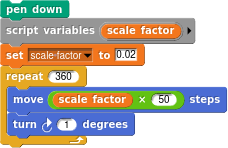
\includegraphics{basicCircle-script.png}
  \end{center}
  \begin{enumerate}
  \item EXPLAIN how this script works as you would like to have it
    explained to you.  Use words, pictures, and so on, as
    needed/helpful in your explanation.

  \item Estimate the RADIUS of this circle to the nearest whole
    number.
    \begin{hint}
      It might help to work with a half-circle and to display
      the turtle's position.
    \end{hint}
  \end{enumerate}

  \begin{freeResponse}
    \begin{enumerate}
    \item So first, we put the pen down. Next we introduce a variable
      called ``scale factor.'' I'm not real sure why. Next we set the
      scale factor to $0.02$ for some reason.

      Now we get to the good part, repeat $360$ times: Forward
      $\mathrm{scale factor}\times 50$ and turn $1$ degree to the
      right.

      At the end of the repeat, we have a circle!

    \item Using the hint, I did this:
      \begin{center}
        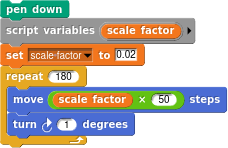
\includegraphics[width=.4\textwidth]{halfCircle-script.png}   \qquad \fbox{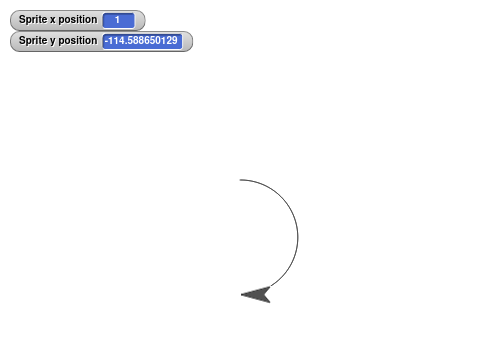
\includegraphics[width=.4\textwidth]{halfCircle-stage.png}}
      \end{center}
      From this I can see that the $y$-position is about
      $-114.589$. Hence the radius is about $57$ units.
    \end{enumerate}
  \end{freeResponse}

  
\end{question}
\mynewpage




\begin{question}
  We would like a circle script that will draw a circle of a given
  radius AROUND a given point. Consider the following \snap\ script:
  
   \adjustbox{valign=t}{
    \begin{tabular}{lp{.4\textwidth}}
      
      \raisebox{-\height}{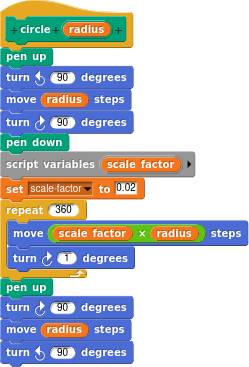
\includegraphics{circle-script.png}}

      &

      While it is similar to the previous script, it has some extra
      features.


      EXPLAIN how this script works as you would like to have it
      explained to you.  Use words, pictures, and so on, as
      needed/helpful in your explanation.  In particular, EXPLAIN what
      the additional blocks are trying to accomplish.
   \end{tabular}}
   \begin{freeResponse}
     The additional blocks are trying (and failing) to make the circle
     centered around the staring point.

     The basic idea is to move the turtle up, draw a circle and then
     move the turtle back down to the center of the circle.
   \end{freeResponse}
\end{question}
\mynewpage



\begin{question}
  Use the bisection method to find a \textbf{scale factor} that will draw a
  circle centered at the turtle's starting point of a given radius.
  Display your work with a table. As a gesture of friendship, I've
  started the table for you:
          \[
          \begin{array}{|c|c|c|c|}\hline
            \text{Attempt} & \text{Scale factor} & \text{Too small or Too large?} \\ \hline\hline
            1 & 0.02 & ?? \\ \hline
            2 & 0.01   & ??  \\ \hline
            \vdots & \vdots & \vdots \\ 
          \end{array}
          \]
  When you are done, display your script, and save your
  circle block so that you can use it again in the future.
  \begin{freeResponse}
    Let's make this table:
    \[
    \begin{array}{|c|c|c|c|}\hline
      \text{Attempt} & \text{Scale factor} & \text{Too small or Too large?} \\ \hline\hline
      1 & 0.02 & \text{too large}  \\ \hline
      2 & 0.01 & \text{too small}  \\ \hline
      3 & 0.015 & \text{too small}  \\ \hline
      4 & 0.0175 & \text{BINGO!}  \\ \hline
    \end{array}
    \]
  
    
     \adjustbox{valign=t}{
       \begin{tabular}{lp{.4\textwidth}}
         
         \raisebox{-\height}{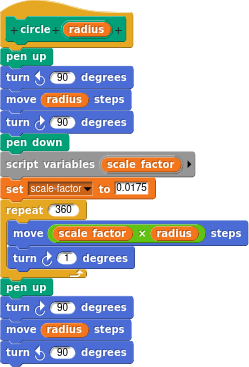
\includegraphics{finalCircle-script.png}}
         
      & Ah ha! This looks like the \snap\ script we want.
   \end{tabular}}
\end{freeResponse}
\end{question}
\mynewpage



\end{document}
